\chapter{Business Model for the Microsoft Kinect Based Exercise Game}
From the information gathered and from the knowledge we have acquired from the research done through this project, we will now structure our work to make an analysis of the business opportunities of the exergame. We will provide a detailed description of a business model that describes how the game should be created and delivered, and how it can create value. As a framework for this description, we will use Osterwalder's Business Model Ontology, as described in chapter 5. \\ \\ 
In this chapter we will describe the potential of Cyberlab's exercise game through all of the nine building blocks.  

\section{Product}
A product covers all aspects of what a company offers to its customers. The product is composed of value propositions, which are services and values offered to the customer. Cyberlab will develop an exercise game used by physiotherapists in prevention and rehabilitation for elderly. The focus of the exercise game is to improve strength and balance in elderly to prevent fall and injuries. The game should have one general workout version directed towards prevention and one customized version used in rehabilitation.
\subsection{Value Proposition}
\emph{A tool with the ability to customize an exercise program and to offer an alternative, fun and motivating training method and at the same time ease the workload of the physiotherapist}\\ \\
Value propositions refer to the value a company offers to a specific customer segment. One value this product provides to the customer is the possibility to offer an alternative, fun and motivating training method. The exercise game is meant to be used as a supplement in training programs or as an exercise motivator. A good motivator is a social aspect, which is highly important for elderly, and that there exist games for different interests. The game can also be used as a tool for physiotherapists to make it easier to customize training programs for their patients. Every patient is different, with individual problems and needs, and it is therefore necessary to provide personalized exercise program for each patient. An important value the product has to serve is that the exercise game can set up training programs and be more motivating than a physiotherapist can. To get a consultation hour at a physiotherapist there is often long waiting lists, so an important aspect for physiotherapists is to be efficient to serve as many patients as possible, without losing quality in the work done. The exercise game can be used to ease the physiotherapists workload. This game has the ability to be a multiplayer game, which makes it possible for physiotherapists to serve more than one player at the same time. A physiotherapist can then consult and exercise with more patients in one hour than a physiotherapist can manage without the exercise game. This will be valuable in the work of shortening the long waiting lists.
\section{Customer Interface}
In this section we will describe how Cyberlab can create value to the customers. Who are the customers, how will they establish contact with them and how will they maintain customer relationship after sales.
\subsection{Customer Segments}
In general, a company generates value for a specific customer segment. To define the right segment for Cyberlab we studied different groups of people; elderly who are them using the exercise game, and several entities related to elderly like training groups, community centres, and physiotherapists.\\ \\ 
\emph{Elderly:}\\ 
The end user of the exercise game are the elderly and they are therefore considered as a possible customer segment. The idea is to sell the game directly to elderly so they can use this exercise game at home. It will be  appealing for this customer segment to have the possibility to exercise at home. The fair of falling makes many elderly afraid of walking outside their own house, and in order to become physically stronger physiotherapy sessions or other appointments once a week is not sufficient. Regular workout at home will contribute to become stronger and increase balance, which prevents falling and increase self confidence. The connection this game has to fun and entertainment in stead of "workout" is a motivating factor to exercise more. A social factor is also included, which is important for elderly who spends much time alone. \\ \\
\emph{Training groups:}\\ 
There exist several training groups focusing on elderly who can be a possible customer segment for Cyberlab. Here, elderly pay a small fee to join a training group, which is fun, social and more motivating than exercising alone. These training groups are engaged by the government, physiotherapy clinics, organizations and individuals. During these workouts this exercise game can be used as a supplement or a different alternative to exercise. Playing the exercise together with other elderly makes the game social and entertaining. \\ \\
\emph{Community centres:} \\
We evaluated community centres for elderly as a possible customer segment. This centres will buy the product and all the equipment needed from Cyberlab and install it in their own environment. With this game they can provide their patients (riktig ord i forhold til eldresenter?) with an alternative activity compared to chess, card play or taking a walk. One possibility for the community centres is to rent out the game to their patients, so the patients can use the equipment for a certain amount of time, alone or in a group. \\ \\
\emph{Physiotherapists:} \\
Physiotherapists is an entity with very close relationship to elderly, and the goal for a physiotherapist is to help elderly decrease the risk of falling by using mobility techniques to improve balance and physical strength. Physiotherapists are also a group of people with a certain authority appearance, which makes them trustworthy. Physiotherapists can buy this product, install it in their environment and use it as a tool for training and in therapy sessions.\\ \\
After composing, studying and discussing business models for each possible customer segment, we recommend Cyberlab to focus on physiotherapy clinics as customers, more precisely, public clinics and private clinics with contribution from the government. The goal of work for a physiotherapist connects well to the purpose of Cyberlab's exercise game, and the authority they have is very valuable when trying to get elderly to adapt the new technology this game provides. The physiotherapy clinics we recommend for Cyberlab has access to a wide customer base consisting of elderly, and they have a stable economy which makes it affordable to buy new products. 

\subsection{Channels}
This subsection about distribution channels describes how Cyberlab should deliver and market their value propositions to the customers. We will describe this by going through the five channel phases.\\ \\
\begin{figure}
\label{fig:Channels}
\begin{center}
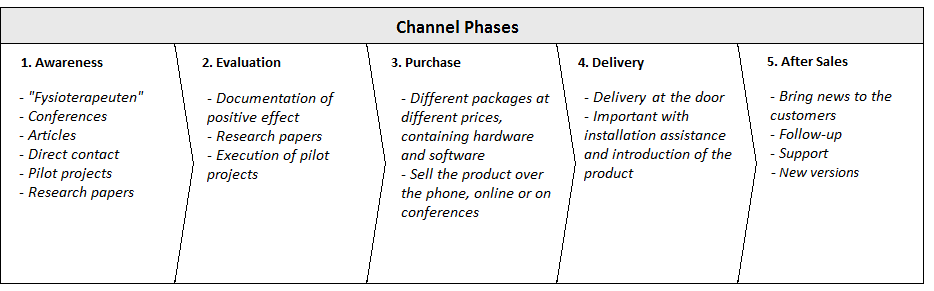
\includegraphics[angle=90,scale=0.7]{channels}
\caption[Channels]{The 5 Channel Phases [modified from \cite{osterwalder}\cite{osterwalderthesis}]}
\end{center}
\end{figure}
\emph{Awareness:} \\ 
We will look into some activities Cyberlab should perform to raise awareness about their product and how they can get their customers attention. "Fysioterapeuten" is a magazine targeting physiotherapists in Norway. This magazine is published by \ac{nff} and distributed out to the whole country. "Fysioterapeuten" contains mostly scientific papers, and the idea is that this magazine shall contribute to evolvement of the physiotherapy profession according to the society and populations need. This magazine is read by 9 000 physiotherapists around the country, and articles printed here are seen as scientific and are therefore taken seriously. Cyberlab should use "Fysioterapeuten" as a medium to promote their exercise game by printing an article or an ad. Printing research papers and articles about the exercise game in other credible magazines or newspapers is also a way to get physiotherapists attention. \\ \\
Another solution for Cyberlab is to promote their product by taking direct contact with target customers. This could be done by joining conferences related to subjects like e.g. welfare technology or by visiting physiotherapy clinics. Cyberlab will then get the opportunity to present the product and show direct interest in establishing a customer relationship. Physiotherapists see it as very relevant to try a product for an amount of time before they decide to buy. When taking direct contact Cyberlab should introduce a suggestion for physiotherapists to run a pilot project, which imply testing the product for free in e.g. 6 months. \\ \\
\emph{Evaluation:}\\
Physiotherapists points out two very important aspects in evaluating a product. These two are; documented effect of the product and own experience by testing the product. If a physiotherapist should even think about trying the product, it is necessary to provide research papers or statistics that shows positive effect in this kind of games. Documentation will give them a security in the choice of buying the product. Other physiotherapists providing positive feedback after trying the game also contributes to this security. Cyberlab should start pilot projects at physiotherapy clinics where physiotherapists will have the possibility to test, experience and evaluate the product themselves for a period of time. The evaluation received from physiotherapists should be used as documentation for the product.\\ \\
\emph{Purchase:} \\
Most physiotherapists have already established connections with suppliers. Ordering and buying products are usually done online, but it can also be by phone or when interesting products are discovered on conferences. Going to the store to buy products is very unusual. To play this game there are software and hardware needed, like Microsoft Kinect sensor and the exercise game. It is unreasonable to think that a physiotherapist already owns a Kinect sensor, so the best strategy for Cyberlab is to sell packages containing both hardware and software. Packages should include various agreements with appropriate pricing. \\ \\
\emph{Delivery:}\\
When buying a new product, especially technical products, there is a need for introduction to the product and maybe also installation assistance. Feedback from interviews with physiotherapists shows the huge importance of start-up help. With much to do at work already, physiotherapists do not have time to pick up deliveries at the postal office, or to setup and learn a new product all by themselves. Buying, receiving, installing and learning should not be difficult or time consuming. \\ \\
From the interviews conducted we found that it was desirable with installation and introduction help when buying technical equipment, so the product should be delivered at the door, by someone who can install the product and teach the physiotherapists how to use it. However, this is a complicated task for Cyberlab if we look at every physiotherapy clinic as their customer segment. It is not realistic that one representative from Cyberlab will travel to the other side of the country as soon as a clinic order the game. Therefore, we will not take this into consideration in this assignment, but there is still an issue to take into account.\\ \\
 
\emph{After sales:}\\
When taking a new product in to use, it is important for physiotherapist to have the possibility to come with feedback. Therefore, Cyberlab should have some kind of support that can take these feedbacks into consideration. Feedbacks can be comments on direct errors or directions on how to make the exercise game more suitable for its use. Cyberlab should follow their customer in the process of learning, and they should inform them of new features and improvements.  
\subsection{Customer Relationships}
Customer relationship is an important part of the customer experience, and it describes what kind of relationship the company establishes with the customers. Support, follow-up and feedback handling are some aspects in establishing customer relationship. Cyberlab has to be available when the customers have problems and need help. When using a new product one may discover errors or find the product not suitable for its use, so many physiotherapists have an eager to provide feedback on this. Cyberlab should handle these feedbacks, fix errors as soon as possible and take comments on improvements into consideration. Using feedback to make a better product shows customers that Cyberlab takes their comments seriously.  In addition, the customers will hopefully get a more suitable product. The maintenance of a direct and personal contact with the customer shows interest in the use and the experience of the product. All this can contribute to a good customer relationship. Cyberlab should also give their customers a heads ups on updates, new features or products.
\section{Infrastructure Management}
This section is about how Cyberlab creates value. What resources needed and what activities that have to be preformed are described here, as well as if they will get them in-house or from a partner. 

\subsection{Key Resources}

In this section we will describe all the resources needed to make the business model work. The resources are divided into 4 different types, described in table \ref{tab:Resources}.
\newpage

\begin{table}
\centering
    \begin{tabular}{|l|l|}
        \hline
       \textbf{Type of Resource} & \textbf{Resource}  \\ \hline
       \emph{Intellectual} & Insight and experience with fall problematic \\ & in elderly \\ \cline{2-2}
        & Programming skills \\ \cline{2-2}
	 	& Creativity \\ \hline
	   \emph{Physical} & Premises \\ \cline{2-2}
	   	& Equipments, i.e. desks and computers  \\ \cline{2-2}
	   	& Microsoft Kinect Sensor \\ \cline{2-2}
	   	& Windows machines \\ \cline{2-2}
	   	& Projector and screen \\ \cline{2-2}
	   	& Working Environment, Kinect for Windows SDK \\ \cline{2-2}
	   	& Internet Connections \\ \hline
	   \emph{Human} & System Developers, i.e. programmers and \\ & interaction designers \\ \cline{2-2}
	   	& Administration, i.e. marketers, customer related \\ &tasks \\ \cline{2-2}
	   	& Support Person(s) \\ \hline
	   \emph{Financial} & The European Union \\
        \hline
    \end{tabular}
    \caption[Resources]{Different types of resources}
    \label{tab:Resources}
\end{table} 
\emph{Intellectual} \\ The developer team needs insight and knowledge about different exercises that will strengthen muscles and improve balance in elderly. Cyberlab is provided with research information from other entities in this project, so their job will be to process this information. When they have enough knowledge to form the foundation of an exercise program, they can start to get creative. Creativity is needed to make the game entertaining and easy to understand and conduct. In addition, good programming competencies are needed to develop the game. To make it as cost-efficient as possible, an experienced team should be put together. \\ \\
\emph{Physical} \\ To be able to conduct this project, the team need premises with everything that comes with it, like desks, chairs, computer, internet connection, lights etc. Cyberlab is an already established business, so we can assume they already have these premises and equipment established, and that this will not provide any additional costs. For this project, they will need specific hardware. The hardware consists of the Kinect sensor, a Windows machine, a server for storing and running the game and a projector and screen for testing purposes. In addition they will need the Kinect for Windows SDK to be able to develop a game for this platform.\\ \\
\emph{Human} \\ Programming skills and creativity are already described above as intellectual resources. So they will need system developers and interaction designers. An administration is needed for marketing, customer related tasks and resource management. When the game is finished it needs to be operated and maintained. These tasks can be done by one or more of the system developers. \\ \\
\emph{Finance} \\ This project is financed by the European Union. However, we will not take this into account when looking at the financial aspects of this game.

\subsection{Key Activities}
The game can be described as a Value Chain, which means transforming inputs into a final product. From the knowledge and experience they have acquired the company wants to make a product as good, cost efficient, and price-competitive so that their customers would choose their product instead of a product with similar value. A description of the different stages in the value chain is depicted in figure \ref{fig:ValueChainCase}. The development of the game should be test-driven, meaning that they will test the product both on the end-users and the customer segment during the development, and adapt the game based on the experiences acquired during the testing. Activities that need to be done include research processing, development, testing, maintenance and updates, support, marketing and administrative tasks, shown in table \ref{tab:activities}. 


\begin{figure}
\begin{center}
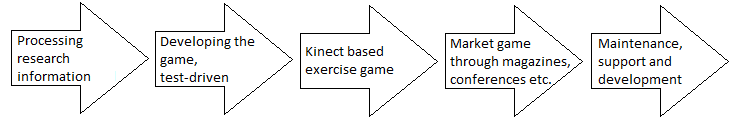
\includegraphics[scale=0.7]{valuechaincase}
\caption[Value Chain for the Kinect Based Exercise Game]{Value chain for the Kinect based exercise game [modified from \cite{osterwalderthesis}]}
\label{fig:ValueChainCase}
\end{center}
\end{figure}

\begin{table}
\centering
    \begin{tabular}{|l|l|}
        \hline
        \textbf{Type of Activity} & \textbf{Activity} \\ \hline
        \emph{Primary} & Research \\ \cline{2-2}
        & Development \\ \cline{2-2}
	 	& Testing \\ \cline{2-2}
	 	& Marketing \\ \cline{2-2}
	 	& Support \\ \hline
	 	 \emph{Support} & Maintenance \\ \cline{2-2}
	   	& Administrative tasks \\
       \hline
    \end{tabular}
    \caption[Different types of activities ]{Different types of activities}
    \label{tab:activities}
\end{table}

\newpage

\subsection{Key Partnerships}
\emph{Microsoft} \\
The main partner in this project is Microsoft. They are the owners of the Kinect sensor for Windows and the SDK. So they have to form some kind of agreement with Microsoft, both on how they can use their hardware and how they can sell it to a third part. \\ \\ 
\emph{Norut} \\
Norut is a national research group located in Tromsø. Cyberlab depends on them because they provide them with research information.  \\ \\ 
\emph{Physiotherapists and the government}\\
Physiotherapists are Cyberlab's customer segment, but they can also serve as a partner. This game fits very well into where the Norwegian health system is going towards (see “Samhandlingsreformen” chapter 3). We mean that this game has a potential to work as a tool for “everyday rehabilitation”. A goal for Cyberlab should be to get this game in as a “regular” tool for prevention and rehabilitation. The government is responsible for the health sector, so they could be a natural partner for the future. Having the government as a partner will solve most of the financial issues. Getting this game into a medical program financed by the government will make this game very credible for the end user. The government could then provide the game to hospitals, care centers, physiotherapy clinics, training groups, and for special cases, when the elderly for example need the game in their own house. \\ \\ 

\section{Financial Aspects}
In this section all the outgoing and incoming money will be described. All the previous blocks described are contributing to a cost or an income. We will try to provide an as realistic and detailed estimate of both costs and income. For convenience we will only consider the Norwegian marked.  (Si noe om v{å}re forutsetninger for {å} kunne beskrive kostnader og inntekter og om forenklingene gjort.)


\subsection{Cost Structure}
Cost structure takes into account all elements that generates costs specific to this game. Cyberlab is an already established business and we can therefore assume that there are not any additional costs associated with premises and some of the "regular" equipment (e.g. desks, chairs, computers etc.). We will not distinguish between fixed and variable costs, but rather look at every costs as fixed annual costs. Variable costs in this case, include installation help, and hardware in stock, because these depend on the demand. For simplification, we will not include these costs here. Other variable costs are salaries associated with support and administrative tasks. Here we will assume that these tasks have assigned a fixed amount of workload for each year. Further, we will distinguish between investment costs and ongoing costs.  \\ \\
\textbf{Investment Costs}\\
Investment costs are all the costs associated with the development of the game. This includes salaries for the development team, the hardware and software needed to develop the game and the cost of the pilot project.  Spending six months on the initial developing and six months on the pilot project, will mean that Cyberlab is looking at a whole year without revenue.\\ \\
\emph{Hardware and Software:}\\
The commercial price for the Kinect sensor is 1790 NOK \cite{pricekinect}, and the \ac{sdk} for the sensor is free. In addition they should have a screen for testing purposes. The screen should be of significant size, so we suggest they invest in a projector and 90" projector screen, which should be sufficient for its purpose. We found that the cost of an average screen lies around 895 NOK and 2449 NOK for a projector \cite{priceprojector}\cite{pricescreen}.\\ \\
\emph{Development:}\\
Cyberlab has estimated that for the developing of this game they need a \ac{fte} = 1.0, meaning that the workload is equivalent to one person working full time for a year. We assume that this will cover development, testing and administrative tasks during the development. In addition, Norut who provides research has also assigned a \ac{fte} = 1.0. How many people assigned to the project is unknown and also irrelevant for the cost prediction, (assuming each employee has the same salary). We have done an estimate on how much the cost of having a engineer with a \ac{fte} = 1 in the private sector is. From \cite{tekna} we found statistics of salary in the private sector in Norway. Assuming that the "average" employer on this project graduated in the end of the 90's, we look at an average gross salary of approximately 730 000 NOK a year. From this we can calculate the average cost of a \ac{fte} = 1.0, based on \cite{altinn}, see Table \ref{tab:costofFTE}, which will be 1 003 349 NOK. We did the same calculations for researchers in the government controlled sector and for marketers in the private sector. They both ended up on a cost of 715 577. See appendix for calculations.\\ \\
\begin{table}
\centering
    \begin{tabular}{|l|l|l|r|}
        \hline
       1&Gross Salary & & 730 000 NOK \\ \hline
       2&Holiday Pay & 12.1\% of 1  & 88 330 NOK \\ \hline
	   3&Employee Fee & 14.1\% of 1+2  & 115 385 NOK \\ \hline
	   4&Pension Costs & 8.0 \% of 1 & 58 400 NOK\\ \hline
	   5&Employee Fee of Pension Costs & 14.1\% of 4 & 8 234 NOK \\ \hline
	   6&Insurance & & 2 000 NOK \\ \hline
	   7&Mobile and Internet & & 1 000 NOK \\ \hline
	   & \textbf{SUM} & & \textbf{1 003 349 NOK} \\
	    \hline
    \end{tabular}
    \caption[Cost of FTE = 1]{The cost of FTE = 1 in the private sector (for Cyberlab}
    \label{tab:costofFTE}
\end{table}
\emph{Pilot Project:}\\
As mentioned we suggest that Cyberlab should run pilot projects to document the effect of the game. This will also serve as a very effective way of marketing the game. We suggest that the pilot project should be carried out in one or more clinics in Trondheim for convenience, and that it should run for six months. The effect have to be documented during the project and after. This documentation should be published in scientific articles and distributed to physiotherapists. We assume that the development of the game will take about six months, so the first year will contain the development phase and the pilot project. The pilot project will most likely provide Cyberlab with valuable feedback on the game, where they can both test the usability in a real environment as well as discover bugs and errors. This will require close monitoring from Cyberlab, so we suggest that this will require a \ac{fte} = 1/5 for this six months (This equals \ac{fte} = 1/10 seen in a whole year). In addition they will have to pay the physiotherapists working with the pilot project. We assume this will be the same amount as their hourly salary. For these six months we will recommend the amount physiotherapists are working with this equal to a FTE=2/5 (or FTE=1/5 seen in a whole year).\\ \\
The investment costs are summarized in table \ref{tab:investmentcosts}. For calculations, see appendix. \\ \\
\begin{table}
\centering
    \begin{tabular}{|l|l|r|}
        \hline
       \textbf{Investment costs}  & &\\ \hline
       Hardware: & & \\ \hline
	   & Kinect sensor & 1 790  \\ \hline
	   & Projector & 2 449 \\ \hline
	   & Screen & 895 \\ \hline
	   Storage & & 1 087 \\ \hline
	   Development team & & \\  
	   FTE=1 &  & 1 003 349   \\ \hline
	   Research from & & \\ 
	   Norut FTE=1 & & 715 577 \\ \hline
	   Pilot Project: & & \\ \hline
	   & Representative(s) from & \\
	   & Cyberlab FTE =1/10 & 100 335  \\ \hline
	   & Representative(s) from & \\
	   & the physiotherapy clinic & \\
	   & FTE = 1/5 & 70 000  \\ \hline
	   \textbf{SUM} & & 1 895 482 
 \\ \hline
    \end{tabular}
    \caption[Investment costs associated to the development of the game]{Investment costs (in \ac{nok}) associated to the development of the game. For calculations on FTE, see appendix}
    \label{tab:investmentcosts}
\end{table}
\newpage
\textbf{Ongoing Costs}\\
We will now look as some ongoing costs on a per year basis. With the rapid evolution of technology, we believe that Cyberlab can offer this game for five years after its release. After, or even during, these years, they will probably have to start making new versions, even for new types of technology. (FINN KILDE PÅ DETTE) We do not take the development of new versions into account in our calculation, and we will set the lifetime of this game to be 5 years.\\ \\
\emph{Storage:}\\
The game has to be operated on a server. This can be on a local server located in Cyberlab’s office, a server located at one of the physiotherapy clinics or on a cloud hosted server. The size of a Kinect game varies a lot, depending on quality, colors, how many levels etc. What we do know is that the game itself will be of fixed size. The dynamic part of the space needed on the server is associated with how many customer profiles it needs to store. This is a hard task to answer, but we assume that the user profiles do not take up that much space, and that Cyberlab can make it with a small server with fixed space. At this stage it is also hard to make an exact assumption on how big the game will become, but from already existing Kinect games, we can assume that the size will not be bigger that 10 GB. From Gogrid Servers \cite{priceserver} we found a small server with storage space of 25 GB. We believe this will be sufficient for Cyberspace's purpose. There is also reasonable to believe that Cyberlab has some space available on their servers. However, if they would have to rent this kind of server space, we are looking at an annual price of \$181.25 which is is roughly 1 087 NOK (with a currency of \$1 = 6 NOK).\\ \\
\emph{Support and Maintenance:}\\
With new software and technology there will always be some errors and bugs after the product or service is delivered. We can assume that the first six months are the most critical months, and will require a \ac{fte} = 1/5. The remaining life time will only need support for some minor problems that might appear (e.g. customer service, operating the server). We assume this period will require a \ac{fte} = 1/10. This is very hard predictable numbers, because this may vary over time. However, our predicted numbers are reasonable as "average" numbers, taking unexpected events into account.  \\ \\
\emph{Marketing:}\\
Marketing is one of the most important part of selling a product or service. This is especially important in the first year of the games life time. The cost of marketing is difficult to analyse because it depends on how long it will take to acquire customers. A new product or services need to acquire customers quickly, and therefore more resources need to be put into the marketing tasks. We can look at the exercise game as a niche product that is targeting a specific customer segment. Thus, the marketing task needs to be customized for this specific customer segment. When a critical mass (the number of customers needed to survive economically in the market) is reached the market will somehow be self-supported \cite{informationrules}. We believe that after this critical phase, the marketing costs will be rather low and close to constant. We assume that the first year right before, during and after the release, the marketing task will contribute to a \ac{fte} = 1/2. After being on the market for one year, the customer base should have reached critical mass.  We believe that in this type of community (the physiotherapist community), words spread fast. If someone starts using a product that is proven good, it will soon appear in magazines and by word of mouth, resulting in the interest from others. Even after critical mass is reached, there will still be some marketing related tasks (e.g. keep up with the market, look for new customer segments), so we suggest that the marketing tasks should contribute to a \ac{fte} = 1/5 after the first year. With this low workload, Cyberlab should consider to hire a marketing consultant instead of having a permanent employee. But in this analysis, we assume they have hired a marketing person for this task. \\ \\
\emph{Costs associated to sales:}\\
The exergame will be sold to the customer as a package with the Kinect sensor and the game included. For convenience, a more comprehensive package with everything else needed to play the game (e.g. screen and a windows machine), should be offered for the interested buyer. here Cyberlab could gain some profit. However, to simplify our calculations we will assume that the package includes the Kinect sensor and the game only and that Cyberlab will not gain any profit on the hardware sold. We will also assume that Cyberlab buy the sensors from Microsoft on demand, meaning they do not have the sensors in stock. This is because of the risk of having a stock. We will discuss this later. Therefore, there are no costs associated to the specific sales. 

\begin{table}
\centering
    \begin{tabular}{|l|r|r|r|r|r|r|}
        \hline
       \textbf{Ongoing costs}  & & & & & & \\ \hline
      \textbf{Year} & \textbf{1} & \textbf{2} & \textbf{3} & \textbf{4} & \textbf{5} & \textbf{Total}\\ \hline
	   Storage & 1 087 & 1 087 & 1 087 & 1 087 & 1 087 &\\ \hline
	  Support & 150 502 & 100 335 & 100 335 & 100 335 & 100 335 & \\ \hline
	  Marketing & 357 789 & 143 115 & 143 115 & 143 115 & 143 115 & \\ \hline
	   \textbf{SUM} & 509 378 & 244 537 & 244 537 & 244 537 & 244 537 & \textbf{935 686} \\ \hline  
	   \textbf{PV} & 489 787 & 226 089 & 217 393 & 209 032 & 200 992 & \textbf{848 380}  \\ \hline
    \end{tabular}
    \caption[Ongoing costs on a per year basis]{Ongoing costs (in \ac{nok}) on a per year basis. For calculations on FTE, see appendix}
    \label{tab:ongoing}
\end{table}
\emph{Total Cost:}\\
Taking all the described costs into account, the project with six years of lifetime (including development and the pilot project) will have a total cost of 2 743 862 NOK.

\begin{table}[h]
\centering
\begin{tabular}{|l|r|}
\hline
\textbf{Total Costs} & \\ \hline
Investment Costs & 1 895 482 \\ \hline
Sum Ongoing Costs PV & 848 380 \\ \hline
\textbf{SUM} & 2 743 862 \\ \hline
\end{tabular}
\caption[Total Costs]{Total Costs in \ac{nok}}
\label{tab:totalcosts}
\end{table}

\subsection{Revenue Streams}
The revenue stream describes how the company can earn money, and for Cyberlab this involves selling a product package consisting of the Microsoft Kinect sensor and the exercise game. There are various ways to sell this product, and we will present two revenue stream solutions.\\ \\
Before pricing the product it is necessary to observe today's market with possible target customers, prices on existing games and physiotherapy tools, and the potential demand for this product. Demand will depend on the documentation of the product and popularity within the physiotherapy community, as well as the product price. Calculating an exact demand for this product is almost impossible due to the lack of existing games in the same genre for this purpose, and also since the game Cyberlab is going to sell does not exist yet. In this section we will assume that the exercise game has been developed, tested and that it has received a great amount of positive feedback. Physiotherapists in Trondheim has started to use the exercise game, and it is being appreciated at the same level as other equipment used at physiotherapy clinics. \\ \\
Pricing the product depends on existing games and tools, and Cyberlabs development costs in hope of achieving a non-negative profit. We start by looking at existing products. Cyberlab's exercise game falls under two definitions, a video game and a tool used in physiotherapy for training and rehabilitation. The video game market today exist of a huge amount of various games. They are mostly in an affordable price range, where e.g. Nintendo Wii games are priced between 99 - 499 NOK \cite{elkjopwii} and Xbox Kinect games are priced between 199 - 399 NOK \cite{elkjopkinect}. Physiotherapy tools has more variation in price range as the definition of this tools are quite wide. Prices can vary from a fixed price of 120 NOK for a stretch pulley \cite{stretchpulley}, 11 000 NOK per month for shockwave therapy leasing (see appendix “Intervju med Nina”), up to 75 000 NOK for a treadmill \cite{treadmill}. As we will present later, a package consisting of hardware and Cyberlab’s exercise game will have a much higher price than other video games on the market. Trying to sell the exercise game for more than the already existing ones will be difficult, so it is therefore highly important for Cyberlab to promote their product as more than just a regular game to justify the price difference. This should be done by emphasizing the products value propositions, which relates the product more to physiotherapy equipment than "just" a video game. \\ \\
Cyberlab’s market potential, which is important to estimate for setting a suitable price, can be roughly calculated by looking at the number of public and private physiotherapy clinics with support from the government, from now on referred to as physiotherapy clinics or just clinics. We looked at four municipalities in Norway; Oslo, Trondheim, Fredrikstad and T{ø}nsberg, where we for each found the number of clinics and compared that number to the population in each municipality. The average ratio we got describe inhabitants per clinic in Norway. Multiplying this with the total population in Norway gave us an approximation of physiotherapy clinics suitable for Cyberlab's customer segment. Our calculation (see Appendix blabla for details) shows that Cyberlab has a possible market in approximately 1 200 physiotherapy clinics in Norway. It should be mentioned that the market potential can become bigger if Cyberlab takes private physiotherapy clinics without any economic support from the government into consideration. These clinics has shown interest in this product, which makes them potential target customers. Also, after some time, when the product has been on the market for a while, physiotherapists has got the time to work with the product and elderly has used the exercise game with assistance in a safe environment, it might be time for Cyberlab to think about expanding their market and start selling the product to end users, the elderly. This will increase the market potential significantly. The package price for the end user has to become drastically lower, and with a greater market potential Cyberlab will have the opportunity to sell their products to a lower and more affordable price for an elderly. Private clinics and elderly will not be taken into consideration when discussing Cyberlab's revenue stream.\\ \\

We will now present two different solution for selling the product, each with proper pricing.\\ \\
\begin{figure}
\label{fig:RevenueStreamPrice}
\begin{center}
\includegraphics[scale=0.8]{revenuestreamprice}
\caption[Price example]{The lowest possible package price Cyberlab can have, provided that they sell the max amount of  copies - 1 200 units, is 2650 NOK}
\end{center}
\end{figure}
\emph{Solution 1 - Fixed price}\\ 
The first solution is to sell the product as a package consisting of both software and hardware to a fixed price. Included in this package is delivery, installation assistance, and introduction to the product. We believe it is necessary  to sell the product included in a total package for several reasons. Assuming that physiotherapy clinics already possesses needed equipment as a Kinect sensor, projector or screens big enough is unreasonable. Neither is it reasonable to believe that physiotherapists will buy software from Cyberlab and then walk to the store to buy rest of the equipment. In the package we have also included installation help and introduction, which we have experienced as important for physiotherapists. For this type of technology equipment it is useful to give an introduction to the product. We can not expect that physiotherapists have the time to teach themselves how the products work. This could result in physiotherapists buying the product and ending up never using it because of the lack of information. \\ \\
The package price will cover hardware needed, and cost connected to development, investment and marketing of the product. The calculated total cost for Cyberlab is approximately 3 170 000 NOK (see Appendix KinesRegneark). This number is only costs related to developing the game, and does therefore not include purchase of hardware for the packages. We will now look at different price proposals for the software, which should cover all costs related to developing the game. A reasonable price for the exercise game, as it can be described as a video game, is a price similar to other video games on the market. The price range of existing Xbox Kinect games are 199 – 399, so we choose to price the game at 300 NOK. How Cyberlab’s revenue will develop with this price is shown in figure (blabla). We observe that Cyberlab has to sell about 10 570 units to cover their total cost, which is an amount almost ten times higher than the estimated market potential. We can therefore conclude that it will be impossible for Cyberlab to sell their game for a price as low as 300 NOK. \\ \\
\begin{figure}
\label{fig:FixedLowPrice}
\begin{center}
\includegraphics[scale=0.7]{fixedlowprice}
\caption[Price related to commercial video games]{Total cost and revenue with price at 300 NOK. We observe that Cyberlab has to sell about 10 570 units to gain some profit}
\end{center}
\end{figure}
If we assume that Cyberlab has the possibility to sell their product to all of the 1 200 physiotherapy clinics in Norway, they could have a price as low as 2 650 NOK, see Figure \ref{fig:RevenueStreamQuantity}, without gaining negative profit. However, it is very risky, almost unreasonable, to assume that Cyberlab could reach out to all target customers. How many units Cyberlab has potential to sell and what price customers are willing to pay depends on demand, which we have mentioned is difficult to measure. A maybe more reasonable sales number would be to cover a third of the possible market share, which is about 400 units. (Si noe om: dette pga av usikkerhet rundt spillet, det er nytt. Ikke alle klinikker har behov. Konservativ gjeng. Ingen lignende teknologi. Ikke s{å} kjent med teknologi).\\ \\
Figure \ref{fig:RevenueStreamPrice} shows three income lines related to three different prices. With a price of 6 000 NOK Cyberlab needs to sell at least 529 units to achieve non-negative profit, but with a price of 10 000 NOK they only has to sell 317 units. Selling to the expected market share, Cyberlab can price these 400 units at 8 000 NOK, which will give Cyberlab a minor profit. However, to also include hardware price in the final package price, the customer will have to pay significantly more for the product. The Kinect sensor, projector and screen costs approximately 5 140 NOK, which means  that the final package price will end up at 13 140 NOK if Cyberlab choose to price their exercise game at 8 000 NOK.\\ \\ 
Figure \ref{fig:RelationPriceAndUnits} shows every combination of price per unit and number of units sold that will cover all of Cyberlab's costs related to developing this exergame, namely 3 170 000 NOK. \\ \\
\begin{figure}
\label{fig:RevenueStreamQuantity}
\begin{center}
\includegraphics[scale=0.7]{revenuestreamquantity}
\caption[Quantity examples]{Total cost and three revenue lines related to three price examples; 6 000 NOK per unit, 8 000 NOK per unit and 10 000 NOK per unit, shows minimum number of units Cyberlab has to sell to achieve a non-negative profit}
\end{center}
\end{figure}

\begin{figure}
\label{fig:RelationPriceAndUnits}
\includegraphics[scale=0.6]{relationpriceandunits}
\caption[Relation between price per unit and number of sold units]{This figure shows every combination of unit price and number of sold units which will cover Cyberlab's total costs}
\end{figure}

\emph{Solution 2 - License agreement}\\
The second solution is to sell the same package as in the first solution, where the package here is implemented in a license agreement. Customers will pay a low start price for the package, and a certain amount of money for each time they use the product. This low start price will not alone cover all of Cyberlab’s total costs, even if they sell to all their potential customers, so it depends on customers using the product. As in the first solution, Installation and introduction is also here included in the package, but it will not be taken into consideration when we describe package price proposals. \\ \\
We will start by making an estimation of how much this exercise game potentially will be used. Usually, a physiotherapist works approximately 8 hours a day, which includes 30 minutes lunch. Not every patient visiting the physiotherapy clinic during a regular day falls under the category “elderly”, and not every elderly visiting the clinic has the need or wants to use this exercise game. We roughly estimate that the exercise game will be used approximately 2 hours a day. A physiotherapist works 47 weeks a year, assuming they have 5 weeks of vacation, and this adds up to 470 hours a year where the exercise game will be used.\\ \\
A proposal for a suitable price for this license agreement is a startup price of 2 000 NOK for the package and a price of 50 NOK (Begrunne denne prisen med total pris for en time, hvor mye de sparer p{å} effektivitet/ha flere i samme time) for each hour physiotherapists use the exercise game. During a year this will add up to 25 500 NOK. In the first solution, the price for hardware was added on top of this total price, but here this is included in the license agreement. Therefore, since Cyberlab’s total costs is measured without consideration of the hardware price we subtract this price from the estimated revenue. So, for each customer purchasing this license agreement, Cyberlab will have an estimated revenue stream of approximately 20 000 NOK. We observe that Cyberlab in this case only need to sell approximately 160 units to make a profit. The income increases much more in this license agreement example than in the fixed price example. Where we in the first example showed that Cyberlab barely achieved profit by selling 400 units, they can with this license agreement sell the same amount of units to a profit of 4 830 000 NOK (See Appendix blabla). \\ \\	
\begin{figure}
\label{fig:RevenueStreamLicense}
\begin{center}
\includegraphics[scale=0.8]{revenuestreamlicense}
\caption[License example]{Profit when using license agreement(blabla}
\end{center}
\end{figure}
We can conclude that selling a license agreement is the best solution for Cyberlab. The possibility of gaining a non-negative profit is higher, and the profit has the potential of becoming much higher than with a fixed price solution. We can conclude that selling a license agreement is the best solution for Cyberlab. The possibility of gaining a non-negative profit is higher, and the profit has the potential of becoming much higher than with a fixed price solution. There will be some risk related to this license agreement. As mentioned, the low startup price for the license agreement is not alone enough to cover all of Cyberlabs costs, so even if Cyberlab manage to cover the whole market they will experience a huge economic loss if no one use the product. Since the idea is that the startup price of 2 000 NOK should cover Cyberlabs costs and the hardware price, we can easily understand that this will lead to a major loss. If we predict that Cyberlab sell the likely amount of 400 units, and no of the customers use the product, they will have a negative profit of - 4 570 000 NOK. However, if all of the 400 customers use the exercise game, only one hour a day for a year will be enough for Cyberlab to gain non-negative profit. Expected life time for a game like this is approximately 5 years, so Cyberlab is actually only dependent on customers using the game one hour a week to gain non-negative profit, which is very likely! (see Appendix blabla2) \\ \\   
For the customers point of view a license agreement will appear more appealing than a fixed package price because of the low startup price (trekke inn noe psykologisk rundt kj{ø}psprosesser). Customers observe that the product price is higher than other existing video games on the market, but they also know what value propositions this exercise game holds, which justify the price difference. They also have information about prices on equipment used at physiotherapy clinics, which makes Cyberlab’s license agreement affordable. Customers also have other reasons for why they prefer this solution. One example is “Ilen Fysioterapi og Idrett”, a private physiotherapy clinic with no economic support from the government, which sees a security in the possibility of buying the product with a license agreement (Se Appendix “intervju med Nina”). The startup price is manageable, and they can control additional costs themselves after how much they want to use the equipment. Private physiotherapists might not have the same financial resources as local institutes, so the idea of paying according to how much they use the product is appealing. 

\subsection{Financial Analysis}
In this section we will make a financial analysis based on the costs and the different revenue streams just described. To be able to see how much revenue we can except each year, we have to make an prediction on how many products can be sold. We suggest that Cyberlab should start with Trondheim as their main focus. The reason for this is that the product has been developed in Trondheim with (close collaboration with the hospital, scientists and physiotherapists?), so the marketing task should be easier. This will make it convenient for Cyberlab to follow up and to respond quickly to requested changes or possible errors.  If Cyberlab can establish a customer base in Trondheim consisting of e.g. 10 physiotherapy clinics and the feedback from these clinics are positive, the game’s reputation will most likely spread to the physiotherapy community in the rest of the country. As we will soon demonstrate, selling the product to 10 physiotherapy clinics to a suitable price will not provide Cyberlab any profit. We believe that as soon as the game gets attention from the rest of the market, it will spin of pretty fast, selling many games, before it will slow down again when the potential market gets saturated. We can describe this with the help of a s-curve, depicted in figure \ref{fig:scurve}. The s-curve describes the diffusion of a product \cite{scurve}. It says something of how an innovation will adopt customers over time. In the introduction of a product or service it will take som time to adopt a critical mass. It is describes as that there are different type of people adopting to the technology described as innovators, early adopters, early majority, late majority, and laggards. As the actors are adopting to the technology, its marked share will eventually have reached all it can takes, meaning it is saturated. Most innovations can be described with a s-curve, but the curve will look different for different innovations. (SI noe om at ordet sprer seg lett? Si noe om vanskeligheter ved {å} spre nye produkter?)\\ \\
  
 \begin{figure}
\begin{center}
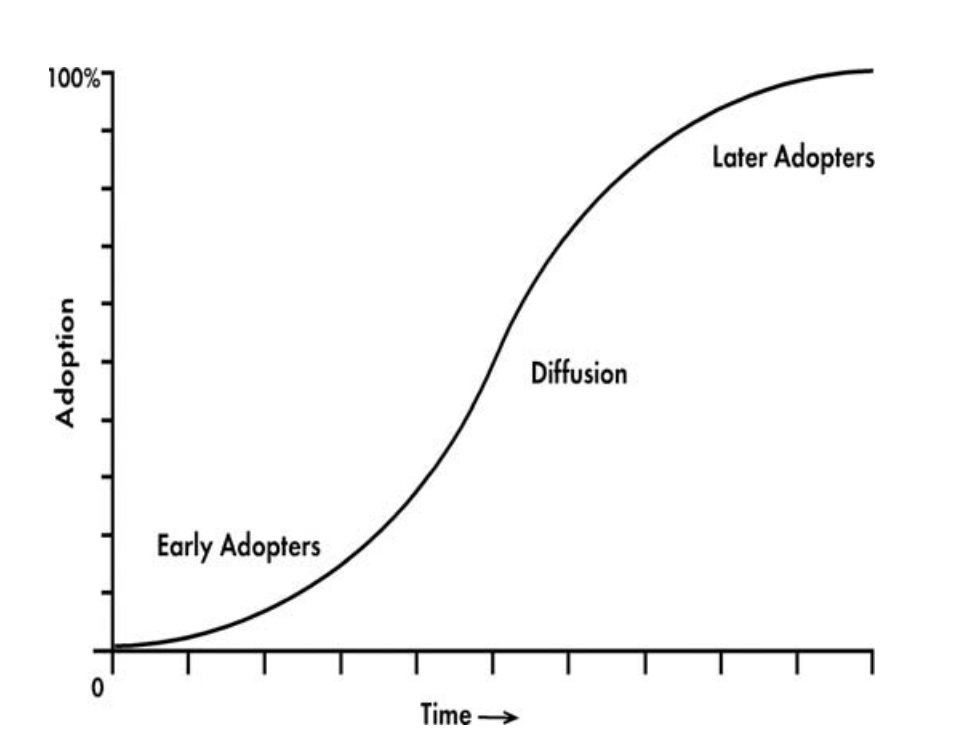
\includegraphics[scale=0.4]{scurve}
\caption[The S-curve]{The S-curve \cite{scurve}}
\label{fig:scurve}
\end{center}
\end{figure}
